\section{A fejlesztési folyamat kiválasztása}

A WatchDB fejlesztési folyamatának kiválasztásánál a projekt mérete, az MVP-re épülő termékstratégia és a későbbi bővíthetőség voltak a legfontosabb szempontok. A korábbi fejezetben bemutatott termékkoncepció alapján az alkalmazás nem egyszerre, teljes funkcionalitással készülne el, hanem először egy szűkített, de használható MVP formájában, majd későbbi verziókban közösségi és haladó funkciókkal bővülne. Ez a felépítés természetesen illeszkedik az iteratív fejlesztési szemlélethez, ahol a csapat kisebb lépésekben halad, és az egyes verziók után visszajelzések alapján pontosíthatja a következő feladatokat \cite{agileManifesto2001}.

A projekt számára ezért egy sprintalapú, de egyszerűsített fejlesztési folyamat tekinthető megfelelőnek. A Scrumhoz hasonlóan a munka időben elkülönített iterációkra bontható, ahol minden sprintnek van egy előre meghatározott célja, például az autentikáció, a filmkeresés, a watchlist vagy a profilnézet elkészítése \cite{schwaberSutherland2020scrumGuide}. Ugyanakkor egy kisebb projekt esetében nem szükséges minden Scrum-eseményt és szerepkört teljes formalitással bevezetni. A hangsúly inkább azon van, hogy a feladatok átláthatóan legyenek priorizálva, a haladás követhető legyen, és minden iteráció végén működő, ellenőrizhető eredmény álljon rendelkezésre.

A fejlesztési folyamat gyakorlati alapját a backlog vagy GitHub Issues jellegű feladatkezelés adhatja. Ide kerülnek a PRD-ből levezetett funkciók, a hibajegyek, a technikai feladatok és a későbbi fejlesztési ötletek. A feladatok prioritizálása az MVP logikáját követi: először azok az elemek kerülnek előtérbe, amelyek nélkül az alkalmazás nem nyújtana önálló értéket, míg a közösségi és kényelmi funkciók későbbi iterációkba sorolhatók.

\begin{figure}[H]
    \centering
    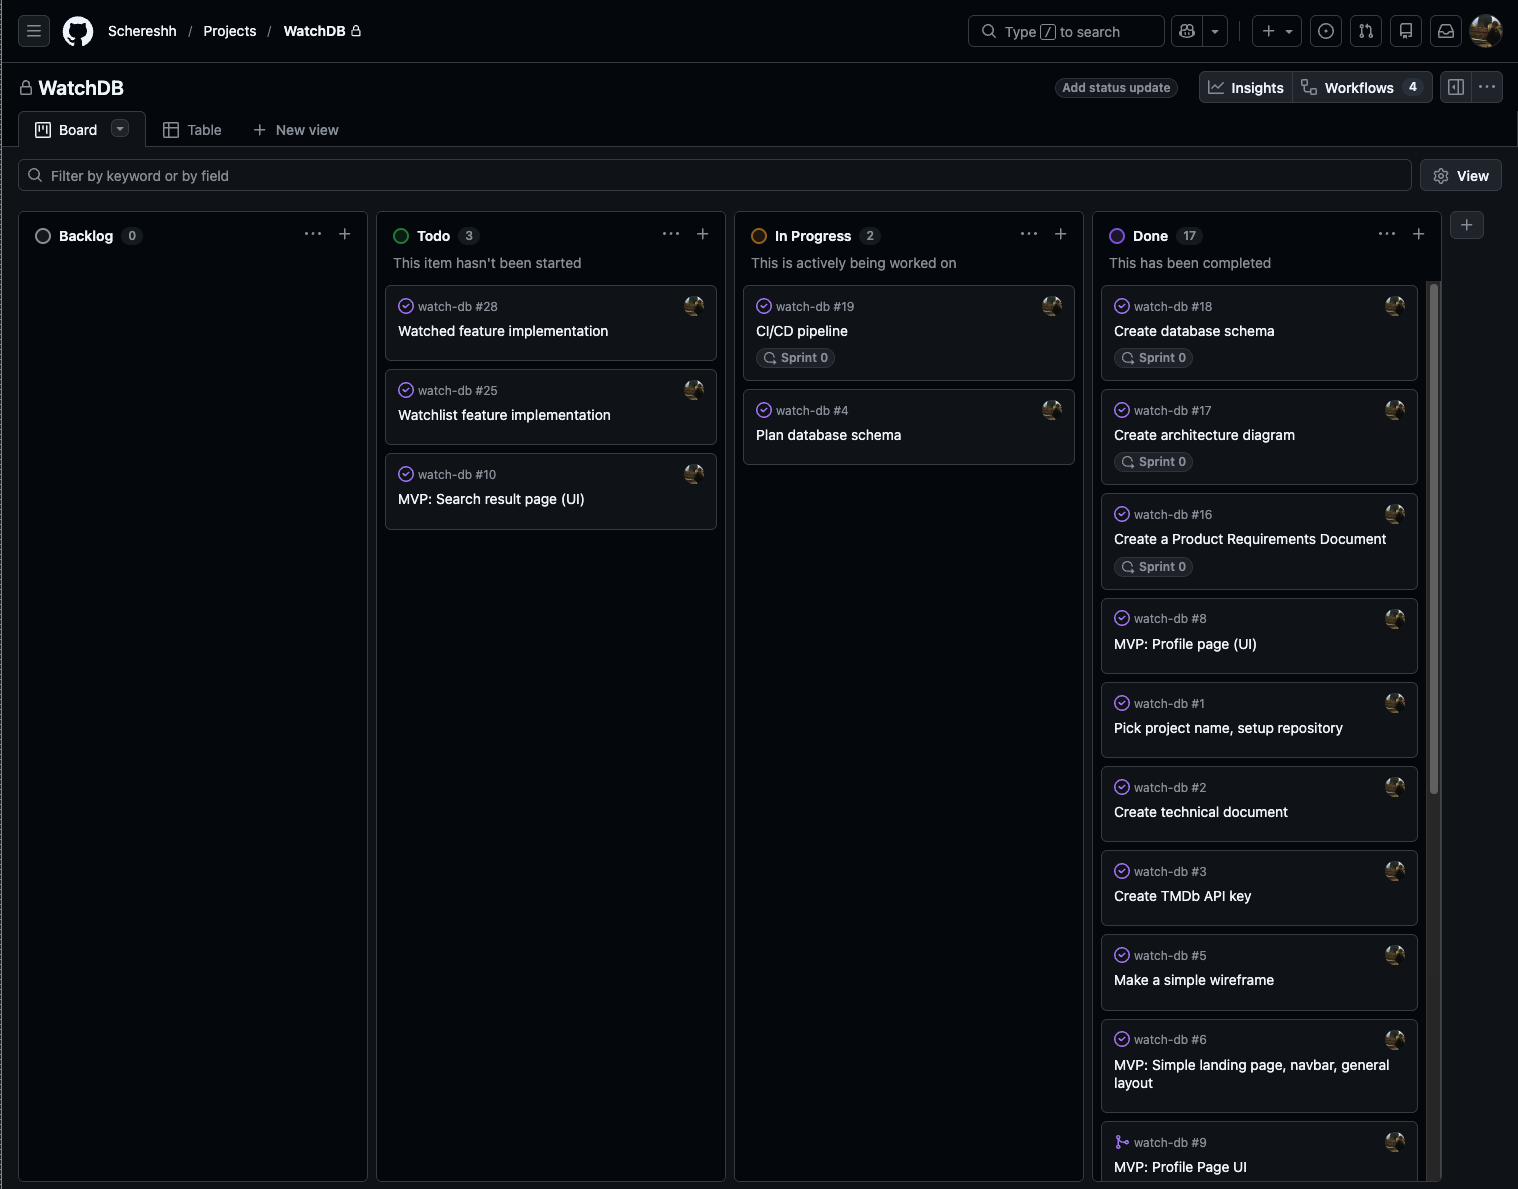
\includegraphics[width=0.92\textwidth]{chapters/chapter-4-developmentProcess/github-projects.png}
    \caption{A WatchDB fejlesztési feladatainak követése GitHub Projects felületen}
    \label{fig:watchdb-github-projects}
\end{figure}

Ez a megközelítés azért előnyös, mert összekapcsolja a terméktervezést és a megvalósítást. A PRD nem különálló dokumentumként marad meg, hanem közvetlenül befolyásolja a backlogot, a sprintek céljait és a fejlesztési sorrendet. Így a projektmenedzsment nem pusztán adminisztratív rétegként jelenik meg, hanem a fejlesztés irányításának gyakorlati eszközeként.
